\section{Superconducting Magnet Controls}
% Following text from Mike Fowler

The Hall C superconducting magnets, power supplies, and cryogenics are
controlled using two redundant pair Programmable Logic Controllers
(PLC). The PLC's are located on the second floor of the Counting
House. They are connected to the the magnets through hot swap analog
and digital IO modules. The IO modules for the High Momentum
Spectrometer (HMS) are also located on the second floor of the
Counting House while the IO modules for the Super High Momentum
Spectrometer (SHMS) are located in the electronics hut on the SHMS
structure in Hall C.

The operator interacts with the controls using the Human Machine
Interface (HMI) console located in the Hall C control room. The HMI
graphically displays the magnet status and allows the operator monitor
the magnet status, adjust the power supply, cryogenics, and remotely
rotate the spectrometers.

The PLC's are programed by and maintained by the Hall C engineering
staff.

% Bunch of sample control screens from Mike Fowler  2/8/2016

\begin{figure}
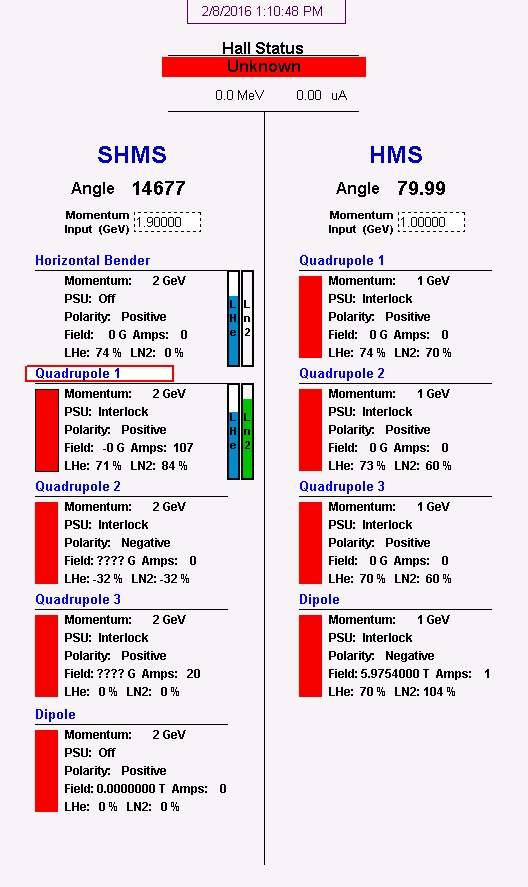
\includegraphics{new_overview}
\caption{\label{fig:magc_overview}Overview of HMS and SHMS magnet status}
\end{figure}

\begin{figure}
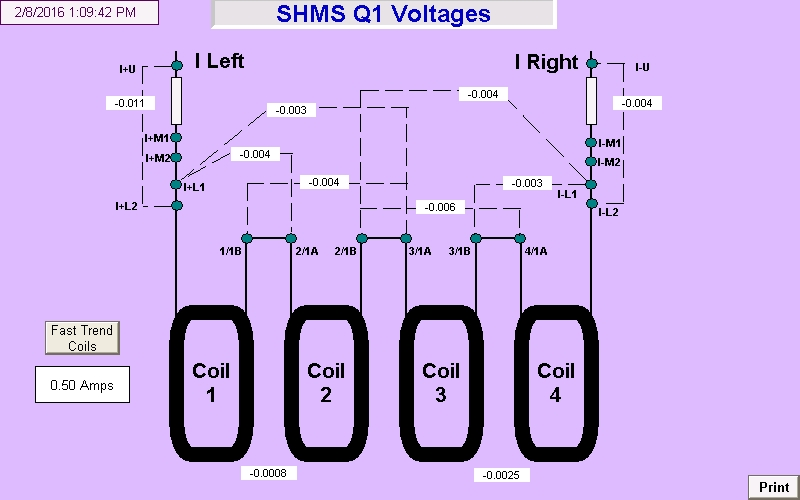
\includegraphics{new_CoilVoltages}
\caption{\label{fig:magc_coilvoltages}SHMS Q1 voltage taps.}
\end{figure}


\begin{figure}
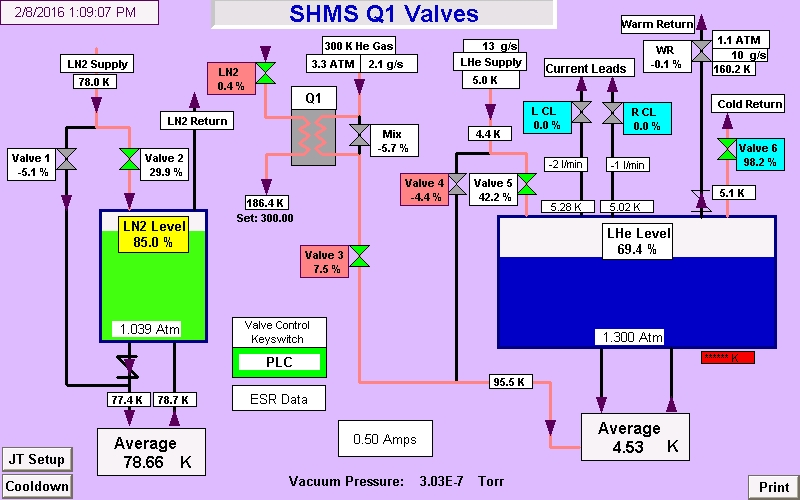
\includegraphics{new_Valves}
\caption{\label{fig:magc_valves}}
\end{figure}


\begin{figure}
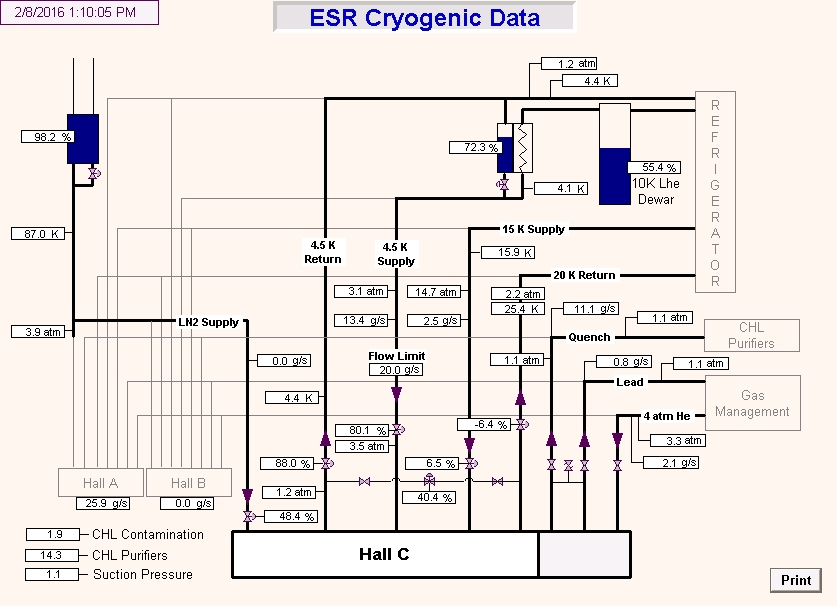
\includegraphics{new_ESR_Data}
\caption{\label{fig:magc_ESR_Data}Status of ESR Cryogenic System}
\end{figure}


\begin{figure}
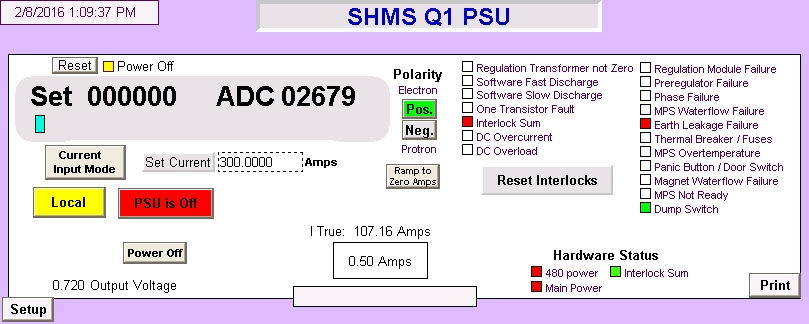
\includegraphics{new_PowerSupply}
\caption{\label{fig:magc_PowerSupply}}
\end{figure}


\begin{figure}
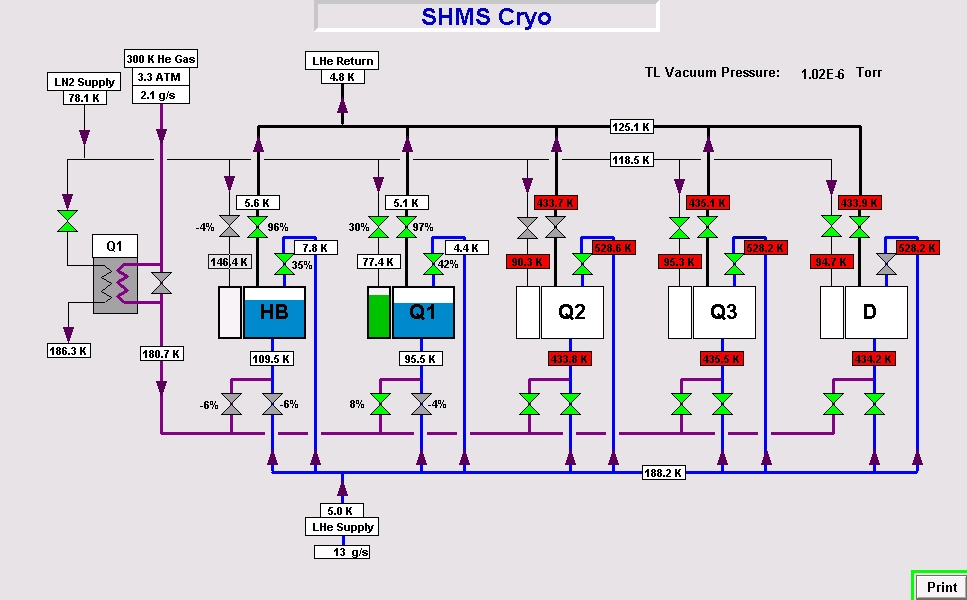
\includegraphics{new_SHMS_Transfer_Line}
\caption{\label{fig:magc_SHMS_Transfer_Line}}
\end{figure}


\begin{figure}
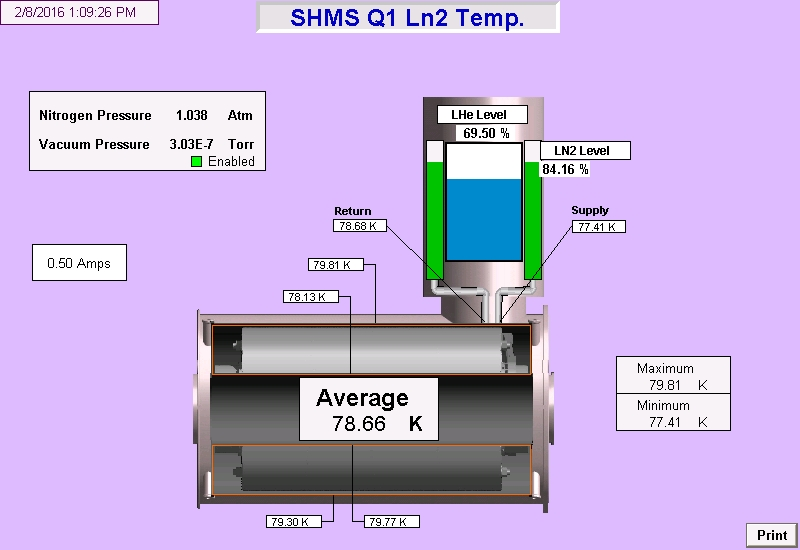
\includegraphics{new_Nitrogen}
\caption{\label{fig:magc_Nitrogen}SHMS Q1 nitrogen temperature and levels}
\end{figure}


\begin{figure}
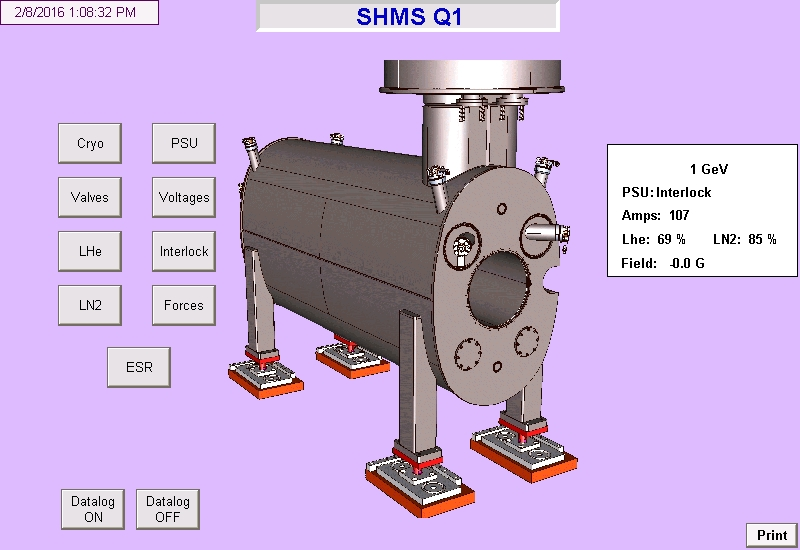
\includegraphics{new_Q1}
\caption{\label{fig:magc_q1}Forces on SHMS Q1 coil packs}
\end{figure}


\begin{figure}
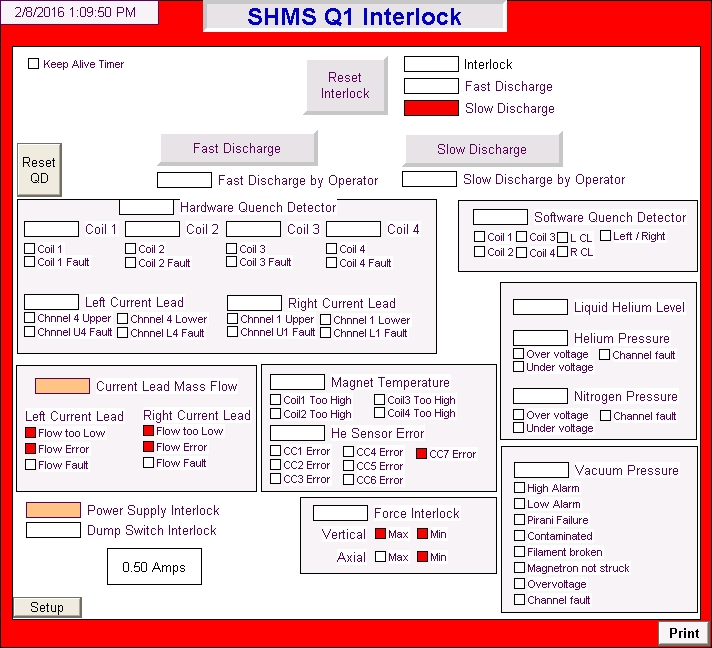
\includegraphics{new_Interlock}
\caption{\label{fig:magc_Interlock}SHMS Q1 power supply interlock status}
\end{figure}


\begin{figure}
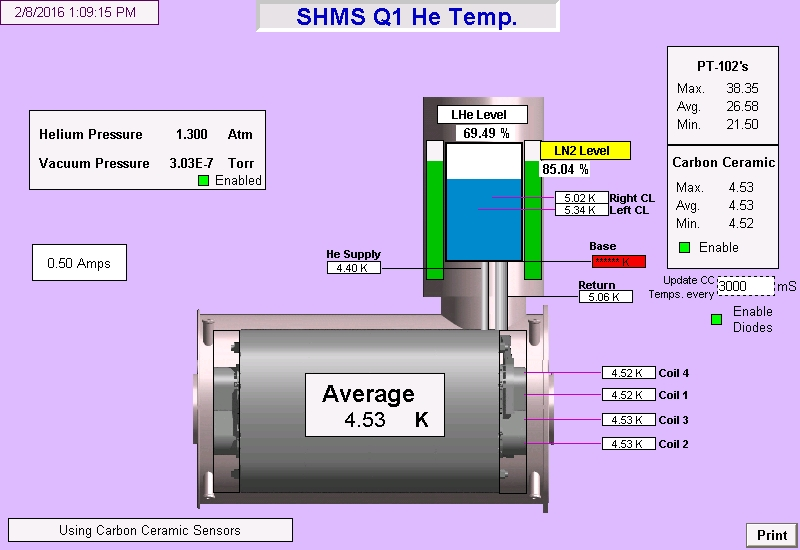
\includegraphics{new_Helium}
\caption{\label{fig:magc_Helium}SHMS Q1 helium temperatures and levels}
\end{figure}





